% Options for packages loaded elsewhere
\PassOptionsToPackage{unicode}{hyperref}
\PassOptionsToPackage{hyphens}{url}
%
\documentclass[
]{book}
\usepackage{amsmath,amssymb}
\usepackage{lmodern}
\usepackage{ifxetex,ifluatex}
\ifnum 0\ifxetex 1\fi\ifluatex 1\fi=0 % if pdftex
  \usepackage[T1]{fontenc}
  \usepackage[utf8]{inputenc}
  \usepackage{textcomp} % provide euro and other symbols
\else % if luatex or xetex
  \usepackage{unicode-math}
  \defaultfontfeatures{Scale=MatchLowercase}
  \defaultfontfeatures[\rmfamily]{Ligatures=TeX,Scale=1}
\fi
% Use upquote if available, for straight quotes in verbatim environments
\IfFileExists{upquote.sty}{\usepackage{upquote}}{}
\IfFileExists{microtype.sty}{% use microtype if available
  \usepackage[]{microtype}
  \UseMicrotypeSet[protrusion]{basicmath} % disable protrusion for tt fonts
}{}
\makeatletter
\@ifundefined{KOMAClassName}{% if non-KOMA class
  \IfFileExists{parskip.sty}{%
    \usepackage{parskip}
  }{% else
    \setlength{\parindent}{0pt}
    \setlength{\parskip}{6pt plus 2pt minus 1pt}}
}{% if KOMA class
  \KOMAoptions{parskip=half}}
\makeatother
\usepackage{xcolor}
\IfFileExists{xurl.sty}{\usepackage{xurl}}{} % add URL line breaks if available
\IfFileExists{bookmark.sty}{\usepackage{bookmark}}{\usepackage{hyperref}}
\hypersetup{
  pdftitle={EST - Estatística},
  pdfauthor={Antônio Neco de Oliveira, Dr.},
  hidelinks,
  pdfcreator={LaTeX via pandoc}}
\urlstyle{same} % disable monospaced font for URLs
\usepackage{longtable,booktabs,array}
\usepackage{calc} % for calculating minipage widths
% Correct order of tables after \paragraph or \subparagraph
\usepackage{etoolbox}
\makeatletter
\patchcmd\longtable{\par}{\if@noskipsec\mbox{}\fi\par}{}{}
\makeatother
% Allow footnotes in longtable head/foot
\IfFileExists{footnotehyper.sty}{\usepackage{footnotehyper}}{\usepackage{footnote}}
\makesavenoteenv{longtable}
\usepackage{graphicx}
\makeatletter
\def\maxwidth{\ifdim\Gin@nat@width>\linewidth\linewidth\else\Gin@nat@width\fi}
\def\maxheight{\ifdim\Gin@nat@height>\textheight\textheight\else\Gin@nat@height\fi}
\makeatother
% Scale images if necessary, so that they will not overflow the page
% margins by default, and it is still possible to overwrite the defaults
% using explicit options in \includegraphics[width, height, ...]{}
\setkeys{Gin}{width=\maxwidth,height=\maxheight,keepaspectratio}
% Set default figure placement to htbp
\makeatletter
\def\fps@figure{htbp}
\makeatother
\setlength{\emergencystretch}{3em} % prevent overfull lines
\providecommand{\tightlist}{%
  \setlength{\itemsep}{0pt}\setlength{\parskip}{0pt}}
\setcounter{secnumdepth}{5}
\usepackage{booktabs}
\usepackage{amsthm}
\makeatletter
\def\thm@space@setup{%
  \thm@preskip=8pt plus 2pt minus 4pt
  \thm@postskip=\thm@preskip
}
\makeatother
\ifluatex
  \usepackage{selnolig}  % disable illegal ligatures
\fi
\usepackage[]{natbib}
\bibliographystyle{apalike}

\title{EST - Estatística}
\author{\href{}{Antônio Neco de Oliveira, Dr.}}
\date{2021-09-13}

\begin{document}
\maketitle

{
\setcounter{tocdepth}{1}
\tableofcontents
}
\hypertarget{estatuxedstica}{%
\chapter{Estatística}\label{estatuxedstica}}

Neste página serão publicadas as anotações da disciplina de estatística para acompanhamento dos encontros síncronos.

Para maiores informações o estudante deverá consultar a bibliografia referenciada.

\includegraphics{./img/simbolo.jpg}

\hypertarget{ementa}{%
\section{Ementa}\label{ementa}}

\begin{itemize}
\item
  A natureza da Estatística, população e amostra. Caracterização de experimentos.
\item
  Definição de probabilidades e o estudo da variável aleatória bem como seus componentes e conceitos.
\item
  Modelos de distribuições discretas de probabilidade e de distribuições contínuas de probabilidade.
\end{itemize}

\hypertarget{objetivos}{%
\section{Objetivos}\label{objetivos}}

\hypertarget{geral}{%
\subsection{Geral}\label{geral}}

\begin{itemize}
\tightlist
\item
  Introduzir aos alunos os conceitos básicos de probabilidade e estatística.
\end{itemize}

\hypertarget{especuxedficos}{%
\subsection{Específicos}\label{especuxedficos}}

\begin{itemize}
\tightlist
\item
  Introduzir o uso de experimento, amostra e população;
\item
  Uso da probabilidade;
\item
  Uso de variável aleatória e distribuições.
\end{itemize}

\hypertarget{conteuxfado-programuxe1tico}{%
\section{Conteúdo Programático}\label{conteuxfado-programuxe1tico}}

\begin{enumerate}
\def\labelenumi{\arabic{enumi})}
\tightlist
\item
  Introdução à estatística.

  \begin{itemize}
  \tightlist
  \item
    Definições estatísticas;
  \item
    População, amostra e evento.
  \end{itemize}
\item
  Conceitos fundamentais.

  \begin{itemize}
  \tightlist
  \item
    Modelos estatísticos;
  \item
    Medidas de tendência central e de variação.
  \end{itemize}
\item
  Análise exploratória de dados.

  \begin{itemize}
  \tightlist
  \item
    Dados, variáveis qualitativas e quantitativas;
  \item
    Distribuições de frequência e representação gráfica;
  \item
    Estimação das medidas de tendência central, de variação e de posição.
  \end{itemize}
\item
  Probabilidade e contagem.

  \begin{itemize}
  \tightlist
  \item
    Espaços amostrais, eventos e operações entre eventos;
  \item
    Probabilidade condicional;
  \item
    Regras da multiplicação e da adição.
  \end{itemize}
\item
  Distribuições discretas de probabilidades.

  \begin{itemize}
  \tightlist
  \item
    Distribuições de Bernoulli, Binomial e de Poisson.
  \end{itemize}
\item
  Distribuições contínuas de probabilidades.

  \begin{itemize}
  \tightlist
  \item
    Distribuição Normal e Normal Padrão.
  \end{itemize}
\item
  Testes de hipóteses.

  \begin{itemize}
  \tightlist
  \item
    Testes unilaterais e bilaterais;
  \item
    Erros de decisão.
  \end{itemize}
\item
  Introdução ao estudo de regressão e correlação:

  \begin{itemize}
  \tightlist
  \item
    Regressão linear simples: estimação dos parâmetros do modelo;
  \item
    Inferências sobre os parâmetros;
  \item
    Correlação.
  \end{itemize}
\end{enumerate}

\hypertarget{metodologia-de-ensino-e-percurso-formativo}{%
\section{Metodologia de ensino e percurso formativo}\label{metodologia-de-ensino-e-percurso-formativo}}

\begin{enumerate}
\def\labelenumi{\arabic{enumi}.}
\item
  Ensino remoto, via ambiente virtual de aprendizagem (Moodle), em concordância com Normas vigentes para a oferta de Carga Horária Semipresencial em Cursos Presenciais do IF Goiano e Regulamento de Oferta de Carga Horária Semipresencial em Cursos Presenciais do IF Goiano -- Campus Morrinhos.
\item
  As aulas serão ministradas nos encontros síncronos dispostos no Ambiente Virtual de Aprendizagem AVA -- Moodle, contendo:

  \begin{enumerate}
  \def\labelenumii{\alph{enumii})}
  \tightlist
  \item
    Slides e textos teóricos sobre o conteúdo ministrado;
  \item
    Fórum para dúvidas;
  \item
    Link para o encontro síncrono via Google Meet;
  \item
    Atividades e questionários para o acompanhamento da aprendizagem.
  \end{enumerate}
\item
  Em cada aula serão apresentados os conceitos teóricos relacionados ao conteúdo em estudo.
\item
  Serão resolvidos exercícios e utilizadas ferramentas eletrônicas para a análise de dados.
\end{enumerate}

\hypertarget{mecanismos-de-atendimento-individualizado-aos-estudantes}{%
\section{Mecanismos de atendimento individualizado aos estudantes}\label{mecanismos-de-atendimento-individualizado-aos-estudantes}}

\begin{itemize}
\tightlist
\item
  Os estudantes deverão primar pela participação em Fóruns, visando o compartilhamento das dúvidas.
\item
  Mandar e-mail para o professor.
\item
  Contudo, será oferecido a possibilidade de agendamento de videoconferências individualizadas ou horários para videoconferências tira-dúvidas.
  E-mail: \texttt{antonio.neco@ifgoiano.edu.br}
\end{itemize}

\hypertarget{forma-nuxfamero-e-crituxe9rios-de-avaliauxe7uxe3o}{%
\section{Forma, número e critérios de avaliação}\label{forma-nuxfamero-e-crituxe9rios-de-avaliauxe7uxe3o}}

\begin{enumerate}
\def\labelenumi{\arabic{enumi})}
\item
  Atividade(s) avaliativa(s):

  \begin{enumerate}
  \def\labelenumii{\arabic{enumii}.}
  \tightlist
  \item
    Avaliações semanais dos conteúdos estudados através de listas de exercícios.
  \item
    Trabalhos avaliativos utilizando erramentas eletrônicas de análise de dados.
  \item
    Cada atividade realizada valerá 10,0 (dez) pontos e a nota final será a média aritmética das notas de todos os trabalhos desenvolvidos no período.
  \item
    Listas de exercícios e questionários, disponibilizados no AVA-Moodle, de acordo com o conteúdo estudado.
  \end{enumerate}
\item
  Feedback da avaliação:

  \begin{itemize}
  \tightlist
  \item
    Ao final de cada atividade avaliativa no Moodle, serão fornecidas as respostas esperadas e a atividade será tema de discussão no encontro virtual seguinte, caso haja dúvidas.
  \end{itemize}
\end{enumerate}

*Essas avaliações poderão ser modificadas, considerando a necessidade de cada turma e/ou o andamento do ano letivo, desde que devidamente esclarecidas para a turma.

\hypertarget{referuxeancias}{%
\section{Referências}\label{referuxeancias}}

\hypertarget{buxe1sica}{%
\subsection{Básica}\label{buxe1sica}}

FONSECA, J. S. \& MARTINS, G.A. Curso de estatística. 6ª ed., São Paulo: Atlas, 1996. 320p.: UFSC, 2003.
BARBETTA, P. A.; REIS, M. M.; BORNIA, A. C. Estatística para cursos de Engenharia e Informática. Editora Atlas, 2004.
CRESPO, A. A. Estatística. São Paulo: Editora Saraiva, 1997.

\hypertarget{complementar}{%
\subsection{Complementar}\label{complementar}}

LAPPONI, J. C. Estatística usando o Excel. São Paulo: Lapponi Treinamento, 2000.
BUSSAB, W. O. \& MORETTIN, P. A. Estatística Básica. Editora Saraiva, 5º edição, 2006.
MURTEIRA, B. Probabilidades e Estatísticas, Vol 1 e 2. Mc Graw-Hill, 1997.
TOLEDO, G. L.; OVALLE, I. L. Estatística Básica. São Paulo: Atlas, 1995.
MORETTIN, P.A. \& BUSSAB, W.O. Métodos Quantitativos. 4ª Ed., São Paulo: Atual Editora Ltda., 1991.

\hypertarget{sugerida}{%
\subsection{Sugerida}\label{sugerida}}

LARSON, R. \& FARBER, B. Estatística aplicada. 6ª ed.~São Paulo: Pearson Education do Brasil, 2015.

\#\citep{barbetta2004estatistica}

\hypertarget{est01---introduuxe7uxe3o}{%
\chapter{EST01 - Introdução}\label{est01---introduuxe7uxe3o}}

All chapters start with a first-level heading followed by your chapter title, like the line above. There should be only one first-level heading (\texttt{\#}) per .Rmd file.

\hypertarget{objetivos-1}{%
\section{Objetivos}\label{objetivos-1}}

\begin{itemize}
\item
  Apresentar os conceitos básicos e o objetivo da estatística.
\item
  Estudar as definições associadas ao estudo de probabilidade.
\end{itemize}

\hypertarget{definiuxe7uxf5es}{%
\section{Definições}\label{definiuxe7uxf5es}}

\hypertarget{probabilidade}{%
\subsection{Probabilidade}\label{probabilidade}}

\begin{itemize}
\item
  A palavra probabilidade deriva do Latim probare (provar ou testar).
\item
  Informalmente, outras palavras são utilizadas para eventos incertos ou conhecidos, como provável, sorte, risco, azar, incerteza, dependendo do contexto.
\item
  A probabilidade é um número que varia de 0 (zero) a 1 (um) e que mede a chance de ocorrência de um determinado resultado.
\item
  Quanto mais próxima de zero for a probabilidade, menores são as chances de ocorrer o resultado e quanto mais próxima de um for a probabilidade, maiores são as chances.
\end{itemize}

\hypertarget{estatuxedstica-1}{%
\subsection{Estatística}\label{estatuxedstica-1}}

\begin{itemize}
\tightlist
\item
  A estatística é uma coleção de métodos para planejar experimentos, obter dados e organizar, resumir, analisar, interpretar e deles extrair conclusões.
\end{itemize}

\hypertarget{introduuxe7uxe3o-uxe0-estatuxedsca}{%
\section{Introdução à Estatísca}\label{introduuxe7uxe3o-uxe0-estatuxedsca}}

Informações divulgadas pelos meios de comunicação provém de pesquisas e estudos estatísticos:

\begin{itemize}
\item
  ``a inflação esse mês foi \ldots."
\item
  ``a taxa de desemprego no Brasil no ano de 2020\ldots."
\item
  ``o candidato A tem 32\% da intenção de votos, o candidato B tem 41\% e 27\% dos entrevistados não souberam ou não quiseram responder"
\item
  ``o número de carros vendidos no país aumentou em 20\%"
\item
  ``a altura média da população aumentou em 5\% "
\item
  ``o time A teve 60\% do tempo de posse de bola, \ldots"
\end{itemize}

\hypertarget{aplicauxe7uxe3o-da-estatuxedstica}{%
\section{Aplicação da Estatística}\label{aplicauxe7uxe3o-da-estatuxedstica}}

Ajudar a responder perguntas do nosso dia a dia, como por exemplo:

\begin{itemize}
\tightlist
\item
  Na compra de 5 bilhetes de uma rifa. Teremos mais chances de ganhar se os números dos bilhetes forem em sequência ou se forem aleatórios?
\end{itemize}

\hypertarget{definiuxe7uxf5es-de-probabilidade}{%
\section{Definições de Probabilidade}\label{definiuxe7uxf5es-de-probabilidade}}

\hypertarget{termos-utilizados-em-probabilidade}{%
\subsection*{Termos utilizados em probabilidade:}\label{termos-utilizados-em-probabilidade}}
\addcontentsline{toc}{subsection}{Termos utilizados em probabilidade:}

\begin{itemize}
\item
  Experimento
\item
  Espaço amostral
\item
  Evento
\item
  Operações entre eventos
\end{itemize}

\hypertarget{probabilidade-1}{%
\subsection{Probabilidade:}\label{probabilidade-1}}

\begin{itemize}
\item
  Estudo da aleatoriedade da incerteza;
\item
  É a quantificação do conhecimento que temos sobre um particular evento.
\end{itemize}

\textbf{Exemplo:}

\begin{itemize}
\tightlist
\item
  Previsão do tempo:
\item
  25\% de probabilidade de chuva.
\item
  Traduz a quantidade de informação que essa pessoa tem da possibilidade, ou não, de chuva.
\end{itemize}

\hypertarget{experimento}{%
\section{Experimento}\label{experimento}}

\hypertarget{determinuxedstico}{%
\subsection{Determinístico:}\label{determinuxedstico}}

\begin{itemize}
\item
  Sempre se repete da mesma forma, apresentando o mesmo resultado.
\item
  Exemplo: soltar uma caneta de uma certa altura;
\item
  Resultado: a caneta vai cair.
\end{itemize}

\hypertarget{aleatuxf3rio}{%
\subsection{Aleatório:}\label{aleatuxf3rio}}

\begin{itemize}
\tightlist
\item
  O resultado do experimento sempre terá um valor diferente.
\item
  Exemplo: Soltar a caneta e medir a distância que ela cai de um determinado local.
\item
  Resultado: a caneta ficará sempre em distância diferente.
\end{itemize}

\hypertarget{espauxe7o-amostral}{%
\section{Espaço Amostral}\label{espauxe7o-amostral}}

\begin{itemize}
\item
  Relação de todos os resultados possíveis de um determinado experimento.
\item
  Denotado pela letra \textbf{S} ou \(\boldsymbol{\Omega}\).
\item
  Exemplo: resultados possíveis no lançamento de um dado.
  \[ S = \{1, 2, 3, 4, 5, 6\} \]
\end{itemize}

\hypertarget{evento}{%
\section{Evento}\label{evento}}

\begin{itemize}
\item
  Subconjunto do espaço amostral.
\item
  Pode ser constituído por um ou mais resultados.
\item
  Exemplo: resultados possíveis no lançamento de um dado cujo valor é ímpar.
  \[ \{1, 3, 5\} \]
\end{itemize}

\hypertarget{operauxe7uxf5es-entre-eventos}{%
\section{Operações entre eventos}\label{operauxe7uxf5es-entre-eventos}}

\hypertarget{uniuxe3o}{%
\subsection{União}\label{uniuxe3o}}

\begin{itemize}
\tightlist
\item
  Acontece \textbf{A} ou \textbf{B} ou os dois.
\end{itemize}

\[A \cup B\]

\begin{figure}

{\centering 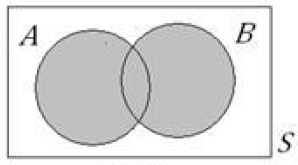
\includegraphics[width=0.25\linewidth]{figuras/uniao} 

}

\caption{União.}\label{fig:unnamed-chunk-1}
\end{figure}

\hypertarget{intersecuxe7uxe3o}{%
\subsection{Intersecção}\label{intersecuxe7uxe3o}}

\begin{itemize}
\tightlist
\item
  Ocorre \textbf{A} e \textbf{B} (os dois) ou todos os eventos.
\end{itemize}

\[A\cap B\]

\begin{figure}

{\centering 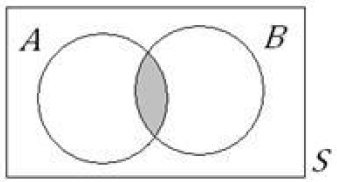
\includegraphics[width=0.25\linewidth]{figuras/interseccao} 

}

\caption{Intersecção}\label{fig:unnamed-chunk-2}
\end{figure}

\hypertarget{evento-complementar}{%
\subsection{Evento Complementar}\label{evento-complementar}}

\begin{itemize}
\tightlist
\item
  Não ocorrência do evento considerado.
  \[\overline{A}\]
  \textbackslash begin\{figure\}
\end{itemize}

\{\centering 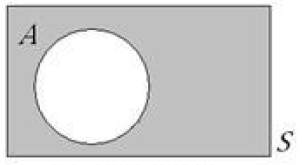
\includegraphics[width=0.25\linewidth]{figuras/complemento}

\}

\caption{Complemento.}

\label{fig:unnamed-chunk-3}
\textbackslash end\{figure\}

\hypertarget{eventos-mutuamente-excludentes}{%
\subsection{Eventos Mutuamente Excludentes}\label{eventos-mutuamente-excludentes}}

\begin{itemize}
\tightlist
\item
  Não possuem nenhum resultado em comum.
  \[A \cap B = \varnothing\]
  \textbackslash begin\{figure\}
\end{itemize}

\{\centering 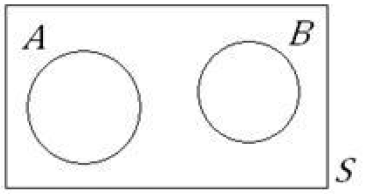
\includegraphics[width=0.25\linewidth]{figuras/excludente}

\}

\caption{Excludente}

\label{fig:unnamed-chunk-4}
\textbackslash end\{figure\}

\hypertarget{definiuxe7uxf5es-de-probabilidade-1}{%
\section{Definições de Probabilidade}\label{definiuxe7uxf5es-de-probabilidade-1}}

\hypertarget{cluxe1ssica}{%
\subsection{Clássica}\label{cluxe1ssica}}

\begin{itemize}
\item
  É a razão entre um número de resultados favoráveis de um evento e o número de resultados prováveis (considerando eventos igualmente prováveis).

  \[ p=\dfrac{m}{n} \]
\item
  \(p =\) probabilidade;
\item
  \(m =\) número de resultados favoráveis;
\item
  \(n =\) número de resultados possíveis.
\end{itemize}

\textbf{Exemplo:} em uma rifa de 100 números, comprado 5, temos:
\[p=\dfrac{5}{100}=5 \% = 0,05 \]

\hypertarget{definiuxe7uxe3o-frequencialista}{%
\subsection{Definição Frequencialista}\label{definiuxe7uxe3o-frequencialista}}

\begin{itemize}
\item
  Para definir probabilidade usa um histórico do que já aconteceu.
\item
  Assume o valor limite de frequência relativa.
\item
  \(\lim_{n\rightarrow \infty} \frac{m}{n}\)
\item
  \(m =\) número de vezes que o evento ocorreu;
\item
  \(n =\) número de experimentos (razoavelmente grande).
\end{itemize}

\hypertarget{definiuxe7uxe3o-axiomuxe1tica}{%
\subsection{Definição Axiomática}\label{definiuxe7uxe3o-axiomuxe1tica}}

Probabilidade é um número associado a um evento que obedece a três leis:

\begin{itemize}
\item
  \(P(E) \geq\) 0;
\item
  \(P(S) = 1\) (probabilidade do evento certo);
\item
  \(P(E \cup F)=P(E) + P(F)\)
\item
  E e F são mutuamente exclusivos;
\item
  Permite desenvolver toda uma teoria a respeito da probabilidade.
\end{itemize}

\hypertarget{definiuxe7uxe3o-subjetiva}{%
\subsection{Definição Subjetiva}\label{definiuxe7uxe3o-subjetiva}}

\begin{itemize}
\item
  Depende da avaliação pessoal;
\item
  Adotada quando não se tem outra forma de atribuir probabilidade;
\item
  Baseada em conceitos prévios de cada um.
\end{itemize}

\textbf{Exemplo:}

\begin{verbatim}
Dois comentaristas esportivos: 

1) O time A ganhará;
2) O vitorioso será o time B. 
\end{verbatim}

\hypertarget{observauxe7uxf5es-gerais}{%
\section{Observações Gerais}\label{observauxe7uxf5es-gerais}}

\begin{itemize}
\tightlist
\item
  \texttt{Clássica:} nem sempre pode ser utilizada.
\end{itemize}

\textbf{Exemplo:} Probabilidade de um avião cair;

\emph{Espaço amostral:} \(S=\{Sim, Não\}\);

\(P=50\%\); ERRO!

\begin{itemize}
\item
  \texttt{Frequencialista:} deve ser aplicada quando o número de eventos tende ao infinito.
\item
  \texttt{Axiomática:} combinação de eventos elementares.
\end{itemize}

\hypertarget{definiuxe7uxf5es-1}{%
\subsection{Definições}\label{definiuxe7uxf5es-1}}

\begin{itemize}
\tightlist
\item
  A probabilidade de eventos complexos será calculada a partir de eventos elementares.
\item
  A probabilidade de eventos elementares será calculada a partir de cada definição. \textbackslash{}
  Clássica (equiprováveis), frequencialista (histórico), subjetiva (nível de informação).
\end{itemize}

\hypertarget{definiuxe7uxf5es-exemplos}{%
\subsection{Definições -- Exemplos}\label{definiuxe7uxf5es-exemplos}}

\begin{itemize}
\tightlist
\item
  Evento: Lançamento de uma moeda \texttt{honesta};
\end{itemize}

Resultado: cara (c) ou coroa (k);

\[p=1/2=0,5 = 50\%\]

\begin{itemize}
\item
  Se a moeda estiver viciada deve-se usar a definição frequencialista.
\item
  Lancei uma moeda ao alto e já tenho o resultado, mas não sei: \(p=0,5\)
\end{itemize}

\hypertarget{lanuxe7amento-feito-para-duas-pessoas-diferentes}{%
\subsubsection*{Lançamento feito para duas pessoas diferentes:}\label{lanuxe7amento-feito-para-duas-pessoas-diferentes}}
\addcontentsline{toc}{subsubsection}{Lançamento feito para duas pessoas diferentes:}

\begin{itemize}
\item
  uma tem aceso ao resultado e responde cara ou coroa: (\(p=1,0\));
\item
  a outra não tem acesso ao resultado e responde cara ou coroa: (\(p=0,5\));
\end{itemize}

\emph{As pessoas estão em estados de informações diferentes.}

\hypertarget{exercuxedcios}{%
\section{Exercícios}\label{exercuxedcios}}

\begin{enumerate}
\def\labelenumi{\arabic{enumi})}
\tightlist
\item
  Em um cassino, localizado em certo país no exterior, o dono providenciou um dado especial. Nesse dado a probabilidade de sair determinado ponto é inversamente proporcional a seu valor.
  Um aluno de Estatística, ao visitar esse cassino, resolveu investigar se estava sendo trapaceado. Com base na observação de diversos eventos, para elaborar um relatório, ele fez os cálculos das probabilidades a seguir.
  Sabendo como o dado se comporta, calcule:
\end{enumerate}

\begin{enumerate}
\def\labelenumi{\alph{enumi})}
\tightlist
\item
  a probabilidade de sair um número menor que 3;
\item
  a probabilidade de sair um número par;
\item
  a probabilidade de sair um número primo;
\item
  a probabilidade de sair ponto 3;
\item
  a probabilidade de sair ponto 6.
\end{enumerate}

\section{Referências}

\% Todas as opções seguintes são opcionais e não são necessárias.
\appendix
\textbackslash section\emph{\{\appendixname\}
\textbackslash subsection}\{Para leitura complementar\}

\begin{frame} %[allowframebreaks]
  \frametitle<presentation>{Referências}
    
  \begin{thebibliography}{10}
    
  \beamertemplatebookbibitems
  % Start with overview books.

  \bibitem{Spiegel_1}
   SPIEGEL, Murray R. 
   \newblock {\em Estatística (3ª edição),}
   \newblock {Pearson 1993.}

  \bibitem{Spiegel_2}
  SPIEGEL, Murray R.
  \newblock {\em Teoria e Probabilidade de Problemas e Estatística (2ª edição),}
  \newblock {Bookman 2004.}
     
   \bibitem{Morettin}
   MORETTIN, Pedro A. \& Bussab, Wilton O. 
   \newblock {\em Estatística Básica (1ª edição),}
   \newblock {Atual 1986.}
   

   
  \beamertemplatearticlebibitems
  % Followed by interesting articles. Keep the list short. 
  \end{thebibliography}
\end{frame}

\hypertarget{anuxe1lise-exploratuxf3ria-de-dados}{%
\chapter{Análise Exploratória de Dados}\label{anuxe1lise-exploratuxf3ria-de-dados}}

\hypertarget{probabilidades}{%
\chapter{Probabilidades}\label{probabilidades}}

\hypertarget{distribuiuxe7uxf5es-discretas-de-probabilidades}{%
\chapter{Distribuições Discretas de Probabilidades}\label{distribuiuxe7uxf5es-discretas-de-probabilidades}}

\hypertarget{distribuiuxe7uxe3o-normal-de-probabilidade}{%
\chapter{Distribuição Normal de Probabilidade}\label{distribuiuxe7uxe3o-normal-de-probabilidade}}

\hypertarget{distribuiuxe7uxe3o-normal-padronizada}{%
\chapter{Distribuição normal padronizada}\label{distribuiuxe7uxe3o-normal-padronizada}}

\hypertarget{testes-de-hipuxf3teses}{%
\chapter{Testes de Hipóteses}\label{testes-de-hipuxf3teses}}

\hypertarget{correlauxe7uxe3o-e-regressuxe3o}{%
\chapter{Correlação e Regressão}\label{correlauxe7uxe3o-e-regressuxe3o}}

  \bibliography{book.bib,packages.bib}

\end{document}
